% \chapter{Sensors}
\chapter{传感器}
\label{chap:sensors}
% Robots are systems that sense, actuate, and compute. So far, we have studied the basic physical principles of actuation, i.e., locomotion and manipulation, and computation, i.e., inverse kinematics and path-planning. We now need to understand the basic principles of robotic sensors that provide the data-basis for computation.

机器人是感知,启动和计算的系统。 到目前为止,我们已经研究了启动的基本物理原理,即运动和操纵以及计算,即反向运动学和路径规划。 我们现在需要了解提供计算数据基础的机器人传感器的基本原理。

% The goals of this chapter are

本章的目标是

\begin{itemize}
% \item provide an overview of sensors commonly used on robotic systems
% \item outline the physical principles that are responsible for uncertainty in sensor-based reasoning

\item 提供了机器人系统常用的传感器概述
\item 概述了基于传感器推理的不确定性的物理原理
\end{itemize}

% \section{Robotic Sensors}
% The development of sensors is classically driven by industries other than robotics. These include submarines, automatically opening doors, safety devices for industry, servos for remote-controlled toys, and more recently the cell-phone, automobiles and gaming consoles. These industries are mostly responsible for making ``exotic'' sensors available at low cost by identifying mass-market applications, e.g., accelerometers and gyroscopes now being used in mass-market smart phones or the 3D depth sensor ``Kinect'' as part of its XBox gaming console. 

\section{机器人传感器}
传感器的发展由机器人以外的行业经典地驱动。 这些包括潜艇,自动开门,工业安全装置,遥控玩具的舵机,以及最近的手机,汽车和游戏机。 这些行业主要负责通过确定大众市场应用程序,例如现在在大众市场智能手机中使用的加速度计和陀螺仪或3D深度传感器“Kinect”作为零件,以低成本制造“异国情调”传感器 的XBox游戏机。

\begin{framed}
% Recap the sensors that you are interacting with daily. What sensors do you have in your phone, in your house and kitchen, or in your car?

重复您每天正在交互的传感器。 你的手机,房屋和厨房里还有什么传感器?
\end{framed}


% As we will see later on, sensors are hard to classify by their application. In fact, most problems benefit from every possible source of information that they can obtain. For example, localization can be achieved by counting encoder increments, but also by measuring acceleration, or using vision. All of these approaches differ drastically in their precision and the kind of data that they provide, but none of them is able to completely solve the localization problem on its own.

% This chapter is therefore organized by the physical quantities (and derivatives thereof), a sensor is measuring, instead of the higher level state estimates it can contribute to. 

如稍后我们将看到的,传感器很难通过其应用进行分类。 事实上,大多数问题受益于他们可以获得的每一个可能的信息来源。 例如,可以通过计数编码器增量,也可以通过测量加速度或使用视觉来实现定位。 所有这些方法在精度和他们提供的数据种类上都有很大的差异,但是它们都不能自行完全解决本地化问题。

因此,本章由物理量(及其衍生物)组织,传感器正在测量,而不是可以对其贡献的较高级别的状态估计。

\begin{framed}
% Think about the kind of data that you could obtain from an encoder, an accelerometer, or a vision sensor on a non-holonomic robot. What are the fundamental differences?

想想可以从非完整机器人的编码器,加速度计或视觉传感器获得的数据种类。 有什么根本的区别?
\end{framed}

% Although an encoder is able to measure position, it is used in this function only on robotic arms. If the robot is non-holonomic, closed tours in its configuration space, i.e., robot motions that return the encoder values to their initial position, do not necessarily drive the robot back to its starting point. In those robots, encoders are therefore mainly useful to measure speed. An accelerometer instead, by definition, measures the derivative of speed. Vision, finally, allows to calculate the absolute position (or the integral of speed) if the environment is equipped with unique features. An additional fundamental difference between those three sensors is the amount and kind of data they provide. An accelerometer samples real-valued quantities that are digitized with some precision. An odometer instead delivers discrete values that correspond to encoder increments. Finally, a vision sensor delivers an array of digitized real-valued quantities (namely colors). Although the information content of this sensor exceeds that of the other sensors by far, cherry-picking the information that are really useful remains a hard, and largely unsolved, problem.

虽然编码器能够测量位置,但仅在机械臂上使用该功能。如果机器人是非完整的,则在其配置空间中的封闭巡视,即将编码器值返回到其初始位置的机器人运动,不一定将机器人驱动回其起始点。因此,在这些机器人中,编码器主要用于测量速度。根据定义,加速度计是衡量速度的导数。如果环境配备了独特的功能,则视觉最终可以计算绝对位置(或速度的积分)。这三种传感器之间的另外的根本区别在于它们提供的数据量和种类。加速度计采集一些精确数字化的实数量。里程表代替传递与编码器增量相对应的离散值。最后,视觉传感器提供数字化的实数数量(即颜色)阵列。尽管传感器的信息内容远远超过了其他传感器的信息,但樱桃采集真正有用的信息仍然是一个难以解决的难题。

% \section{Proprioception of robot kinematics and internal forces}
% \emph{Proprioception} \index{Proprioception} refers to the perception of internal states of a robot. 
% This is different from \emph{exteroception}\index{Exteroception}, which describes sensing of anything outside of the robot. Proprioception includes awareness of the robot's joint angles, its speeds, as well torques and forces.

% The main internal sensor is therefore the encoder. Encoders can be used for sensing joint position and speed, as well as --- when used together with a spring --- a simple force sensor. There are both incremental and absolute encoders. The latter are mostly used in industrial applications, but are not common in mobile robotics. There are magnetical and optical encoders, which both rely on a magnetic or optical beacon turning together with the motor and being sensed by an appropriate sensor that counts every pass-through. The most common encoder in robotics is the optical \emph{quadrature encoder} \index{Quadrature encoder}. It relies on a pattern rotating with the motor and an optical sensor that can register black/white transitions. Whereas those patterns can be precision manufactured, simple encoders can be made by simply laser-cutting a pattern such as shown in Figure \ref{fig:encoders} and reading it with a light sensor.

\section{机器人运动学和内力的本体感觉}
\emph{Proprioception}\index{Proprioception}是指对机器人的内部状态的感知。
这与\emph{exteroception}\index{Exteroception}有所不同,它描述了对机器人以外的任何东西的感测。本体感觉包括对机器人关节角度,速度以及转矩和力的认识。

因此,主内部传感器是编码器。编码器可用于感应关节位置和速度,以及---与弹簧一起使用时-简单的力传感器。有增量和绝对编码器。后者主要用于工业应用,但在移动机器人中并不常见。存在磁光编码器和光学编码器,它们都依赖于与电动机一起转动的磁性或光学信标,并且由适当的传感器感测到,该传感器对每次通过进行计数。机器人中最常见的编码器是光学\emph{quadrature encoder}\index{Quadrature encoder}。它依赖于与电机旋转的图案和可以注册黑/白转换的光学传感器。虽然这些图案可以精确制造,但简单的编码器可以通过简单地激光切割如图1所示的图案来制作,并用光传感器读取。

\begin{figure}
	\centering
		\includegraphics[width=0.3\textwidth]{figs/encoderdisk.png}
		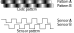
\includegraphics[width=0.3\textwidth]{figs/quadraturencoder.png}
		\includegraphics[width=0.3\textwidth]{figs/absoluteencoder.png}
	% \caption{From left to right: encoder pattern used in a quadrature encoder, resulting sensor signal (forward motion), absolute encoder pattern (gray coding).}
	\caption{从左到右:在正交编码器中使用的编码器模式,产生传感器信号(前向运动),绝对编码器模式(灰色编码)。}
	\label{fig:encoders}
\end{figure}

% While a single sensor would be sufficient to detect rotation and its speed, it does not allow for the determining the direction of motion. Quadrature encoders therefore have two sensors, A and B, that register an interleaving pattern with distance of a quarter phase. If A leads B, for example, the disk is rotating in a clockwise direction. If B leads A, then the disk is rotating in a counter-clockwise direction. It is also possible to create absolute encoders, an example of which is shown in Figure \ref{fig:encoders}, right. This pattern encodes 3-bits, encoding 8 different segments on a disc. Notice that the pattern is arranged in such a way that there is only one bit changing from one segment to the other. This is known as ``Gray code''\index{Gray code}. The function of linear encoders is analogous, both for incremental and absolute encoders.

% If combined with a spring, such as in a series elastic actuator, rotary and linear encoders can be used as simple force/torque sensors using Hooke's law ($F=kx$, force equals distance times spring constant). Whereas the series elastic actuator is the most illustrative examples, most load cells operate on the premise of measuring displacements within materials of known properties. Here, measuring changes in resistance or capacitance might be easier choices.

% Other means of measuring the actual force at the end-effector or joint torques is measuring the actual current consumed at each joint. Knowing a mechanism's pose allows to calculate the resulting forces and torques across the mechanism as well as the currents required for empty loading conditions. Derivations of these then correspond to additional forces that can hence be calculated.

% Finally, there are other means of proprioception, such as simple sensors that can detect when a robot gets picked up, e.g.
 
当单个传感器足以检测旋转及其速度时,它不允许确定运动方向。因此,正交编码器具有两个传感器A和B,其以四分之一相位的距离对交织模式进行注册。例如,如果A引导B,则盘沿顺时针方向旋转。如果B引导A,则盘沿逆时针方向旋转。也可以创建绝对编码器,其示例如图\ref{fig:encoders}所示。该模式编码3位,在光盘上编码8个不同的段。请注意,模式的布置方式是只有一个位从一个区段更改为另一个区段。这被称为“格雷码”,“指纹格雷码”。线性编码器的功能类似于增量式和绝对式编码器。

如果与一个弹簧(如串联弹性执行机构)结合使用,旋转和线性编码器可用作简单的力/扭矩传感器,使用胡克定律($F=kx$,力等于距离乘以弹簧常数)。尽管串联弹性致动器是最具说明性的示例,但是大多数称重传感器在测量已知特性材料内的位移的前提下工作。在这里,测量电阻或电容的变化可能更容易选择。

测量末端执行器或关节扭矩时的实际力的其他方法是测量每个关节消耗的实际电流。了解机构的姿态允许计算机构上所产生的力和扭矩以及空载条件所需的电流。然后,这些导数对应于可以计算的附加力。

最后,还有其他的本体感觉手段,例如可以检测何时拾取机器人的简单传感器,例如。


% \section{Sensors using light}
% The small form factor and low price of light-sensitive semi-conductors have led to a proliferation of light-based sensing relying on a multitude of physical effects. These include reflection, phase shift, and time of flight.

\section{传感器使用光}
光敏半导体的小尺寸和低价格导致了基于大量物理效应的光传感器的扩散。 这些包括反射,相移和飞行时间。

% \subsection{Reflection}
% Reflection is one of the principles that is easiest to exploit: the closer an object is, the more it reflects light shined at it. This allows to easily measure distance to objects that reflect light well and are not too far away. In order to make these sensors as independent from an object's color (but unfortunately not totally independent), infrared is most commonly chosen. A distance sensor is made from two components: an emitter and a receiver. They work by emitting an infrared signal and then measuring the strength of the reflected signal. A typical response is shown in Figure \ref{fig:epuckir}. The values obtained at an analog-digital converter correspond to the voltage at the infrared receiver and are saturated for low distances (flat line), and quadratically fall off thereafter.

\section{反射}

反思是最容易利用的原则之一:对象越接近,它反射的光越多。这允许轻松测量距离反射光的物体的距离,而不是太远。为了使这些传感器独立于物体的颜色(但不幸的是并非完全独立的),最常选择红外线。距离传感器由两个部件组成:发射器和接收器。它们通过发射红外信号然后测量反射信号的强度来工作。典型的响应如图\ref{fig:epuckir}所示。在模拟数字转换器处获得的值对应于红外接收器处的电压,并且对于低距离(扁平线)是饱和的,并且此后二次掉下来。


\begin{figure}
	\centering
		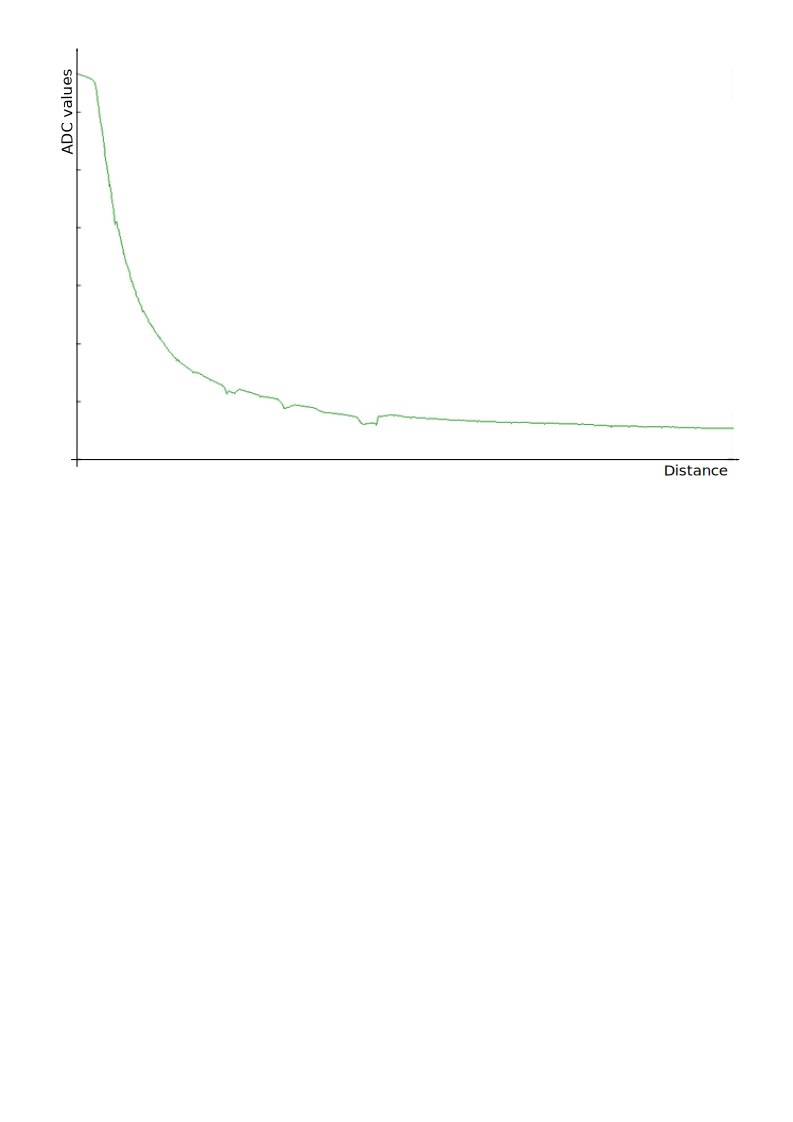
\includegraphics[width=0.8\textwidth]{figs/epuckirsensor.png}
	% \caption{Typical response of an infrared distance sensor as a function of distance. Units are left dimensionless intensionally.}
	\caption{作为距离的函数的红外距离传感器的典型响应。单位是无量纲的。}
	\label{fig:epuckir}
\end{figure}

% When using more than one infrared sensor/emitter pair, e.g., using a camera and a projector not only allows to measure the distance of many points at once, but also to assess the structure of the environment by calculating its impact on the deformation of patterns. For example a straight line becomes a curve when projected onto a round surface. This approach is known as \emph{structured light}\index{Structured light} and illustrated in Figure \ref{fig:struclight}. Thanks to the continuously increasing efficiency of computational systems, a light-weight version of such an approach has become feasible to be implemented at small scale and low cost at around 2010, and emerged as a novel standard in robotic sensing.

当使用多个红外传感器/发射器对时,例如使用照相机和投影仪,不仅可以一次测量多个点的距离,还可以通过计算其对图案变形的影响来评估环境的结构。例如,当投影到圆形表面上时,直线变为曲线。这种方法被称为\emph{structure light}\index{Structured light},如图\ref{fig:struclight}所示。由于计算系统的效率不断提高,这种方法的轻量化版本在2010年左右以小规模,低成本实现已成为可行,并成为机器人传感的新标准。

\begin{figure}
	\centering
		\includegraphics[width=\textwidth]{figs/structuredlight.png}
	% \caption{From left to right: two complex physical objects, a pattern of colored straight lines and their deformation when hitting the surfaces, reconstructed 3D shape. From \protect\cite{zhang2002rapid}.}
	\caption{从左到右:两个复杂的物体,一条彩色直线的图案及其在表面上的变形,重建了3D形状。 From \protect\cite{zhang2002rapid}.}
	\label{fig:struclight}
\end{figure}

% Instead of using line patterns, infrared-based depth image sensors use a speckle pattern (a collection of randomly distributed dots with varying distances), and two computer vision concepts: \emph{depth from focus} and \emph{depth from stereo}.\index{Depth from Focus}\index{Depth from Stereo} When using a lens with a narrow focal depth, objects that are closer or farther away appear blurred (you can easily observe this on professional portrait photos, which often use this effect for aesthetic purposes). Measuring the ``bluriness'' of a scene (for known camera parameters) therefore allows for an initial estimate of depth. Depth from stereo instead works by measuring the disparity of the same object appearing in two images taken by cameras that are a known distance apart. Being able to identify the same object in both frames allows to calculate this disparity, and from there the distance of the object. (The farther the object is away, the smaller is the disparity.) This is where the speckle pattern comes in handy, which simply requires to search for blobs with similar size that are close to each other.

基于红外线的深度图像传感器不使用线条图案,而是使用斑点图案(随机分布的不同距离点的集合)和两个计算机视觉概念:\emph{depth from focus}和\emph{depth from stereo}。\index{深度从焦点}\index{深度从立体声}当使用具有较窄焦距的镜头时,更近或更远的物体显得模糊不清(您可以很容易地观察到专业人像照片,通常使用此效果审美目的)。因此,测量场景的“模糊度”(对于已知的摄像机参数)可以初步估计深度。通过测量出现在已知距离相机的相机拍摄的两张图像中的相同物体的差异,可以使立体声的深度代替。能够在两个框架中识别相同的对象允许计算该差异,并从那里距离对象的距离。(物体离开越远,差距越小。)这是散斑图案派上用场的地方,只需要搜索相似尺寸的斑点即可。


% \subsection{Phase shift}
\subsection{相移}
\label{sec:phaseshiftsensors}

% As you can see in Figure \ref{fig:epuckir}, reflection can only be precise if distances are short. Instead of measuring the strength (aka amplitude) of the reflected signal, laser distance sensors measure the phase difference of the reflected wave. In order to do this, the emitted light is modulated with a wave-length that exceeds the maximum distance the scanner can measure. If you would use visible light and do this much slower, you would see a light that keeps getting brighter, then getting darker, briefly turns off and then starts getting brighter again. Thus, if you would plot the amplitude, i.e. its brightness, of the emitted signal vs. time you would see a wave that has zero-crossings when the light is dark. As light travels with the speed of light, this wave propagates through space with a constant distance (the wavelength) between its zero crossings. When it gets reflected, the same wave travels back (or at least parts of it that get scattered right back). For example, modern laser scanners\index{Laser range finder} emit signals with a frequency of 5 MHz (turning off 5 million times in one second). Together with the speed of light of approximately 300,000km/s, this leads to a wavelength of 60m and makes such a laser scanner useful up to 30m.

% When the laser is now at a distance that corresponds exactly to one half the wave-length, the reflected signal it measures will be dark at the exact same time its emitted wave goes through a zero-crossing. Going closer to the obstacle results in an offset that can be measured. As the emitter knows the shape of the wave it emitted, it can calculate the phase difference between emitted and received signal. Knowing the wave-length it can now calculate the distance. As this process is independent from ambient light (unless it has the exact same frequency as the laser being used), the estimates can be very precise. This is in contrast to a sensor that uses signal strength. As the signal strength decays at least quadratically, small errors, e.g. due to fluctuations in the power supply that drives the emitting light, noise in the analog-digital converter, or simply differences in the reflecting surface have drastic impact on the accuracy and precision (see below for a more formal definition of this term). 

% As the laser distance measurement process is fast, such lasers can be combined with rotating mirrors to sweep larger areas, known as \emph{Laser Range Scanners}\index{Laser Range Scanners}. Such systems have been combined into packages consisting of up to 64 scanning lasers, providing a depth map around a car while driving, e.g. It is also possible to modulate projected images with a phase-changing signal, which is the operational principle of early ``time-of-flight'' cameras, which is not an accurate description of their operation, however.


从图中可以看出,如果距离很短,反射只能是精确的。激光距离传感器不是测量反射信号的强度(又称振幅)而是测量反射波的相位差。为了做到这一点,发射的光被调制,波长超过扫描仪可以测量的最大距离。如果你使用可见光,做得这么慢,你会看到光线不断变亮,然后变暗,短暂关闭,然后再次变亮。因此,如果您将绘制发射信号的幅度即其亮度与时间相比较,则会在光线较暗时看到具有过零点的波形。当光以光速行进时,该波在其零交叉之间以恒定距离(波长)传播通过空间。当它被反射时,相同的波浪返回(或至少部分地区散落在后面)。例如,现代激光扫描仪\index{激光测距仪}发射频率为5 MHz的信号(在一秒内关闭500万次)。连同光速约30万公里/秒,这导致波长为60米,使这样的激光扫描仪可达30米。

当激光器现在处于与波长的一半正好相当的距离时,其测量的反射信号在其发射波经过过零点的同时会变暗。靠近障碍物导致可以测量的偏移。当发射器知道其发射的波形时,可以计算发射和接收信号之间的相位差。知道波长,现在可以计算距离。由于该过程独立于环境光(除非具有与所使用的激光器完全相同的频率),所以估计可以非常精确。这与使用信号强度的传感器相反。信号强度至少二次衰减,小误差,例如,由于驱动发光的电源的波动,模拟数字转换器中的噪声或反射表面的简单差异对精度和精度有很大的影响(参见下文关于该术语的更正式定义)。

随着激光距离测量过程的快速化,这种激光器可以与旋转镜组合以扫描较大的区域,称为\emph{激光测距扫描仪(Laser Range Scanners)}\index{激光测距扫描仪(Laser Range Scanners)}。这样的系统已被组合成由多达64个扫描激光器组成的包装,在驾驶时提供围绕汽车的深度图,例如。然而,也可以用相位改变信号调制投影图像,这是早期“飞行时间”摄像机的操作原理,但这并不能准确描述它们的操作。


% \subsection{Time-of-flight}
% The most precise distance measurements light can provide is by measuring its time of flight. This can be done by counting the time a signal from the emitter becomes visible in the receiver. As light travels very fast (3,000,000,000m/s), this requires high-speed electronics that can measure time periods smaller than nano-seconds in order to achieve centimeter accuracy. In practice this is done by combining the receiver with a very fast (electronic) shutter that operates at the same frequency with which light is emitted. As this timing is known, one can infer the time light must have been traveling by measuring the quantity of photons that have made it back from the reflective surface within one shutter period. Considering a concrete example, light travels 15m in 50ns. Therefore, it will take a pulse 50ns to return from an object at a distance of 7.5m. If the camera sends out a pulse of 50ns length and then closes the receiver with a shutter, the receiver will receive more photons the closer the object is, but no photons if the object is farther away than 7.5m. Given a fast enough and precise circuit that acts as a shutter, it is sufficient to measure the actual amount of light that returns from the emitter.


\subsection{飞行时间}
光线可以提供的最精确的距离测量是通过测量其飞行时间。这可以通过计数来自发射器的信号在接收器中变得可见的时间来完成。当光线速度快(3,000,000,000m/s)时,这需要高速电子设备,可以测量小于纳秒的时间,以达到厘米的精度。实际上,这是通过将接收机与以相同频率工作的非常快速(电子)快门组合来完成的。在这个时刻已知的情况下,可以通过测量在一个快门期间内从反射表面返回的光子的量来推断出光必须行进的时间。考虑一个具体的例子,光在50ns内行进15m。因此,距离7.5米距离的物体需要50ns的脉冲。如果相机发出长度为50ns的脉冲,然后用快门关闭接收器,则接收器将接收到物体越近的更多光子,但如果物体距离物体远离7.5m,则无光​​子。给出一个足够快速且精确的电路作为快门,足以测量从发射器返回的实际光量。


% \section{Sensors using sound}
% \subsection{Ultra-sound distance sensors}
% Ultra-sound distance sensor: An ultra-sound distance sensor operates by emitting an ultra-sound pulse and measures its reflection. Unlike a light-based sensor that measures the amplitude of the reflected signal, a sound-based sensor measures the time it took the sound to travel. This is possible, because sound travels at much lower speed (300m/s) than light (300,000km/s). The fact that the sensor actually has to wait for the signal to return leads to a trade-off between range and bandwidth. (Look these definitions up above before you read on.) In other words, allowing a longer range requires waiting longer, which in turn limits how often the sensor can provide a measurement. Although US distance sensors have become less and less common in robotics, they have an advantage over light-based sensors: instead of sending out a ray, the ultra-sound pulse results in a cone with an opening angle of 20 to 40 degrees. By this, US sensors are able to detect small obstacles without the requirement of directly hitting them with a ray. This property makes them the sensor of choice in automated parking helpers in cars.

\section{传感器使用声音}
\subsection{超声距离传感器}
超声距离传感器:超声距离传感器通过发出超声波脉冲来测量其反射。与测量反射信号的幅度的基于光的传感器不同,基于声音的传感器测量声音行进的时间。这是可能的,因为声音以比光(300,000km/s)低得多的速度(300m/s)行进。传感器实际上必须等待信号返回的事实导致范围和带宽之间的折衷。(在阅读之前,先看看这些定义)换句话说,允许更长的距离需要等待更长时间,这又限制了传感器提供测量的频率。虽然美国距离传感器在机器人技术中越来越少见,但它们比基于光的传感器具有优势:而不是发出光线,超声波脉冲产生的开口角为20至40度的锥体。由此,美国传感器能够检测小障碍物,而不需要用射线直接击中它们。这个属性使他们成为汽车自动停车助手的首选传感器。


% \subsection{Texture recognition}
% Audible sound consists of high frequency vibrations in the range between 20 Hz and roughly 15 kHz. Microphones are therefore ideally suited to measure vibrations in this range. This allows them to double as the Pascinian corpuscle in human skin cells, which is known to have a resonance frequency of 250 Hz and is mostly responsible for texture recognition. Indeed, rubbing a texture against a microphone can indeed be used for differentiating between tens and hundreds of different textures \cite{hughes14}, with a number of commercial sensors available. These sensors usually calculate the frequency spectrum of the recorded signal, which can then be classified using machine learning techniques. Being able to recognize a texture by touch is important in applications like grasping and navigation through cluttered terrain.  

\subsection{纹理识别}
声音由20Hz至15kHz范围内的高频振动组成。因此,麦克风非常适合测量此范围内的振动。这使得它们可以像人类皮肤细胞中的帕斯克氏球体一样增加,已知其具有250Hz的共振频率,并且主要负责纹理识别。事实上,摩擦麦克风的纹理确实可以用于区分数十和数百种不同纹理\cite{hughes14},有许多商业传感器可用。这些传感器通常计算记录信号的频谱,然后可以使用机器学习技术进行分类。能够通过触摸识别纹理在诸如抓住和穿过杂乱地形的导航中的应用中是重要的。


% \section{Inertia-based sensors}
% A moving mass does not loose its kinetic energy, but for friction. Likewise, a resting mass will resist acceleration. Both effects are due to ``inertia'' \index{Inertia} and can be exploited to measure acceleration and speed. 

% \subsection{Accelerometer}
% An accelerometer \index{Accelerometer}can be thought of as a mass on a dampened spring. Considering a vertical spring with a mass hanging down from it, we can measure the acting force $F=kx$ (Hooke's law) \index{Hooke's law}by measuring the displacement $x$ that the mass has stretched the spring. Using the relationship $F=am$, we can now calculate the acceleration $a$ on the mass $m$. On earth, this acceleration is roughly $9.81\frac{kg m}{s^2}$. In practice, these spring/mass systems are realized using microelectromechanical systems (MEMS), such as a cantilevered beam whose displacement can be measured, e.g., using a capacitive sensor. Accelerometers measure up to three axes of translational accelerations. Infering a position from this requires integration twice, thereby amplifying any noise, making position estimates using accelerometers alone infeasible. As gravity provides a constant acceleration vector, accelerometers are very good at estimating the pose of an object with respect to gravity.

\section{基于惯量的传感器}
移动的质量不会松动其动能,而是摩擦。同样,静止的质量将抵抗加速。这两种效应都是由于'惯性''\index{惯性}而且可以用来测量加速度和速度。

\subsection{加速度计}
加速度计\index{加速度计}可以被认为是一个潮湿的弹簧上的质量。考虑到垂直弹簧与其下垂的质量,我们可以通过测量质量已经拉伸的位移$x$来测量作用力$F=kx$(胡克定律)\index{胡克定律}。使用关系$F=am$,我们现在可以计算质量$m$的加速度$a$。在地球上,这个加速度大概是$9.81\frac{kgm}{s^2}$。实际上,这些弹簧/质量系统使用微机电系统(MEMS)实现,例如可以例如使用电容传感器来测量其位移的悬臂梁。加速度计测量多达三个平移加速度的轴。从这个位置推算需要两次集成,从而放大任何噪音,使用单独加速度计的位置估计是不可行的。当重力提供恒定的加速度矢量时,加速度计非常好地估计物体相对于重力的姿态。


% \subsection{Gyroscopes}
% A gyroscope is an electro-mechanical device that can measure rotational orientation. It is complementary to the accelerometer that measures translational acceleration. Classically, a gyroscope consists of a rotating disc that could freely rotate in a system of pivots and gimbals. When moving the system, the inertial momentum keeps the original orientation of the disc, allowing to measure the orientation of the system relative to where the system was started. A variation of the gyroscope is the rate gyro, which measures rotational speed. 

% What a rate gyro \index{Rate gyro}\index{Gyroscopes} measures can most intuitively be illustrated by considering the implementation of an \emph{optical} rate gyro. In an optical gyro, a laser beam is split into two beams and send around a circular path in two opposite directions. If this setup is rotated against the direction of one of these laser beams, one laser will have to travel slightly longer than the other, leading to a measurable phase-shift at the receptor. This phase shift is proportional to the \emph{rotational speed} of the setup. As light with the same frequency and phase will add, and lights with the same frequency but opposite phases will cancel each other, light at the detector will be darker for high rotational velocities. As small-scale optical rate gyros are not practical for multiple reasons, MEMS rate gyros rely on a mass suspended by springs. The mass is actively vibrating, making it subject to Coriolis forces, when the sensor is rotated. Coriolis forces can be best understand by moving orthogonally to the direction of rotation on a vinyl disk player. In order to move in a straight line, you will not only need to move forwards, but also sideways. The necessary acceleration to change the speed of this sideway motion is counteracting the Coriolis force, which is both proportional to the lateral speed (the vibration of the mass in a MEMS sensor) and the rotational velocity, which the device wishes to measure. Note that the MEMS gyro would only be able to measure acceleration if it were not vibrating.

% Gyroscopes can measure the rotational speed around three axes, which can be integrated to obtain absolute orientation. As an accelerometer measures along three axes of translation, the combination of both sensors can provide information on motion in all six degrees of freedom. Together with a magnetometer (compass), which provides absolute orientation, this combination is also known as \emph{Inertial Measurement Unit} (IMU), \index{Inertial Measurement Unit}\index{IMU}.


\subsection{陀螺仪}
陀螺仪是可以测量旋转方向的机电装置。它是测量平移加速度的加速度计的补充。经典地,陀螺仪由可在枢轴和万向节系统中自由旋转的旋转盘组成。当移动系统时,惯性动量保持盘的原始方向,允许测量系统相对于系统启动位置的方向。陀螺仪的一个变化是测量转速的速率陀螺仪。

通过考虑执行一个\emph{optical}速率陀螺仪,可以最直观地说明陀螺仪\index{率陀螺仪}\index{陀螺仪}测量值。在光学陀螺仪中,将激光束分成两束,并以两个相反的方向绕圆形路径传送。如果这个设置是按照这些激光束之一的方向旋转的,那么一个激光器将不得不比另一个激光器稍微延长,导致受体处的可测量的相移。该相移与设置的\emph{转速}成比例。由于具有相同频率和相位的光将增加,并且具有相同频率但相反相位的光将彼此抵消,因此在高旋转速度下,检测器的光将变暗。由于小尺度光学速率陀螺仪由于多种原因是不实际的,因此MEMS速率陀螺仪依靠由弹簧悬挂的质量。当传感器旋转时,质量块正在积极振动,使其受到科里奥利力的影响。通过与乙烯基盘播放器上的旋转方向垂直移动,可以最好地了解科里奥利力。为了直线移动,您不仅需要向前移动,而且还需要向前移动。改变这种侧向运动速度的必要加速度抵消科里奥利力,其与横向速度(MEMS传感器中的质量的振动)和设备希望测量的旋转速度成正比。请注意,如果MEMS陀螺仪不振动,则只能测量加速度。

陀螺仪可以测量围绕三个轴的旋转速度,可以集成以获得绝对定向。作为加速度计沿着三个平移轴测量,两个传感器的组合可以提供所有六个自由度的运动信息。与提供绝对方位的磁力计(罗盘)一起,这种组合也称为\emph{惯性测量单位}(IMU),\index{惯性测量单位}\index{IMU}。


% \section{Beacon-based sensors}
% Localizing an object by triangulation goes back to ancient civilizations orienting themselves using the stars. As stars are only visible during unclouded nights, seafarers have eventually invented systems of artificial beacons emitting light, sound, and eventually radio waves. The most sophisticated of such systems is the Global Positioning System (GPS). GPS consists of a number of satellites in orbit, which are equipped with knowledge about their precise location and have synchronized clocks. These satellites broadcast a radio signal that travels at the speed of light and is coded with its time of emission. GPS receivers can therefore calculate the distance to each satellite by comparing time of emission and time of arrival. As not only the position (x,y,z), but also the time difference between the GPS receiver's clock and the synchronized clocks of the satellites is unknown, four satellites are needed to obtain a ``fix''. Due to the way information from the satellites is coded, getting an initial fix can take in the order of minutes, but eventually is available multiple times a second. GPS measurements are neither precise nor accurate enough (see below) for small mobile robots, and require to be combined with other sensors, such as IMUs and compasses. (The bearing shown on some GPS receivers is calculated from subsequent positions and is therefore meaningless if the robot is not moving.) 

% There exist also a variety of indoor-GPS solutions, which consists of either active or passive beacons that are mounted in the environment at known locations. Passive beacons, for example infrared reflecting stickers arranged in a certain pattern or 2D barcodes, can be detected using cameras and their pose can be calculated from their known dimensions. Active beacons instead usually emit radio, ultrasound or a combination thereof, which can then be used to estimate the robot's range to this beacon. 


\section{基于信标的传感器}
通过三角测量来定位对象可以追溯到古代文明中,使用星星。由于星星只在昏昏沉沉的夜晚可见,海员们最终发明出发光,声音和最终无线电波的人造信标系统。这些系统中最复杂的是全球定位系统(GPS)。GPS由轨道上的许多卫星组成,它们具有关于其精确位置的知识并具有同步时钟。这些卫星广播以光速行进的无线电信号,并以其发射时间进行编码。因此,GPS接收机可以通过比较发射时间和到达时间来计算每个卫星的距离。不仅位置(x,y,z),而且GPS接收机的时钟和卫星的同步时钟之间的时差也是未知的,需要四颗卫星来获得“固定”。由于来自卫星的信息被编码,获得初始修复可以采取几分钟的顺序,但最终可以多次可用。GPS测量对于小型移动机器人来说既不准确也不准确(见下文),并且需要与其他传感器(如IMU和罗盘)组合。(某些GPS接收器上显示的轴承是从后续位置计算出来的,如果机器人不动,则无效)。

还存在各种各样的室内GPS解决方案,其中包括安装在已知位置的环境中的主动或被动信标。可以使用照相机检测被动信标,例如以某种图案或2D条形码布置的红外反射贴纸,并且可以从其已知尺寸计算其姿态。主动信标通常发射无线电,超声波或其组合,然后可以用它来估计机器人到该信标的范围。


% \section{Terminology}
% It is now time to introduce  a more precise definition of terms such as ``speed'' and ``resolution", as well as additional taxonomy that is used in a robotic context. 

\section{术语}
现在是时候引入更为精确的术语定义,如“速度”和“分辨率”,以及在机器人环境中使用的附加分类法。

%% Was Commented
%Roboticists differentiate between proprioceptive and exteroceptive sensors. Proprioceptive sensors measure quantities that are internal to the robot such as wheel-speed, current consumption, joint position or battery status. Exteroceptive sensors measure quantities from the environment, such as distance to a wall, the strength of ambient light or the pattern of a picture at the wall.
%% Was Commented


% Roboticists differentiate between \emph{active} and \emph{passive} sensors. Active sensors \index{Active sensor} emit energy of some sort and measure the reaction of the environment. Passive sensors \index{Passive sensor} instead measure energy from the environment. For example, most distance sensors are active sensors (as they sense the reflection of a signal they emit), whereas an accelerometer, compass, or a push-button are passive sensors.

% The difference between the upper and the lower limit of the quantity a sensor can measure its known as its \emph{range}~\index{Range (sensor)}. This should not be confused with the \index{Dynamic Range (sensor)} \emph{dynamic range}, which is the ratio between the highest and lowest value a sensor can measure. It is usually expressed on a logarithmic scale (to the basis 10), also known as ``decibel''\index{Decibel}. The minimal distance between two values a sensor can measure is known as its \index{Resolution (sensor)} \emph{resolution}. The resolution of a sensor is given by the device physics (e.g., a light detector can only count multiples of a quant), but usually limited by the analog-digital conversion process. The resolution of a sensor should not be confused with its accuracy or its precision (which are two different concepts). For example, whereas an infrared distance sensor might yield 4096 different values to encode distances from 0 to 10cm, which suggests a resolution of around 24 micrometers, its precision is far above that (in the order of millimeters) due to noise in the acquisition process.


机器人主义者区分\emph{active}和\emph{passive}传感器。主动传感器\index{Activesensor}发射某种能量,并测量环境的反应。被动传感器\index{被动传感器}代替测量环境中的能量。例如,大多数距离传感器是有源传感器(因为它们感测到它们发射的信号的反射),而加速度计,罗盘或按钮是无源传感器。

传感器可以测量其数量的上限和下限之间的差值,称为其\emph{range}〜\index{Range(sensor)}。这不应该与传感器可以测量的最高和最低值之间的比例\index{动态范围(传感器)}\emph{动态范围}相混淆。它通常以对数刻度(基于10)表示,也称为“decibel”\index{Decibel}。传感器可以测量的两个值之间的最小距离称为其\index{Resolution(sensor)}\emph{resolution}。传感器的分辨率由器件物理学(例如,光检测器只能计数量子的倍数)给出,但通常受模拟数字转换过程的限制。传感器的分辨率不应与其精度或精度(这是两个不同的概念)混淆。例如,红外距离传感器可能产生4096个不同的值来编码从0到10cm的距离,这表示大约24微米的分辨率,其精度远高于由于采集过程中的噪声引起的(毫米数量级)。


% Technically, a sensors accuracy \index{Accuracy (sensor)} is given by the difference between a sensors (average) output $m$ and the true value $v$:

传感器精度\index{精度(传感器)}由传感器(平均值)输出$ m $和真值$ v $之间的差值给出:

\begin{equation}
accuracy=1-\frac{|m-v|}{v}
\end{equation}

% This measure provides you with a quantity that approaches one for very accurate values and zero if the measurements group far away from the actual mean. In practice, however, this measure is only rarely used and accuracy is provided with absolute values or a percentage at which a value might exceed the true measurement. 

% A sensor's precision \index{Precision (sensor)} instead is given by the ratio of range and statistical variance of the signal. Precision is therefore a measure of repeatability of a signal, whereas accuracy describes a systematic error that is introduced by the sensor physics. This is illustrated in Figure \ref{fig:precision}.


如果测量组远离实际平均值,此度量值为您提供接近于非常准确值的数量,并且为零。然而,实际上,这种措施很少使用,准确性是提供绝对值或一个值可能超过真实测量的百分比。

传感器的精度\index{Precision(传感器)}由信号的范围和统计方差的比值给出。因此,精度是信号重复性的度量,而精度描述了由传感器物理学引入的系统误差。这在图\ref{fig:precision}中说明。


\begin{figure}
	\centering
		\includegraphics[width=0.9\textwidth]{figs/precisionvsaccuracy.png}
	% \caption{From left to right, the cross corresponds to the true value of the signal: neither precise nor accurate, precise but not accurate, accurate but not precise, accurate and precise. 
	\caption{从左到右,十字对应于信号的真实值:既不精确也不准确,精确但不准确,准确但不准确,准确和准确。
	\label{fig:precision}}
\end{figure}

% A GPS sensor is usually precise within a few meters, but only accurate to tens of meters. This becomes most obvious when satellite configurations change, resulting in the precise region jumping by a couple of meters. In practice, this can be avoided by fusing this data with other sensors, e.g. from an IMU.

% The speed at which a sensor can provide measurements is known as its \index{Bandwidth (sensor)} \emph{bandwidth}. For example, if a sensor has a bandwidth of 10 Hz, it will provide a signal ten times a second. This is important to know, as querying the sensor more often is a waste of computational time and potentially misleading.


GPS传感器通常在几米内精确,但精确到数十米。当卫星配置改变时,这变得最明显,导致精确的区域跳跃几米。实际上,这可以通过将这些数据与其他传感器融合来避免这种情况。来自IMU。

传感器可以提供测量的速度称为其\index{带宽(传感器)}\emph{bandwidth}。例如,如果一个传感器的带宽为10赫兹,它将提供一秒钟的信号十次。这很重要,因为更频繁地查询传感器是浪费计算时间和潜在的误导。


% \section*{Take-home lessons}
\section*{课后补充}
\begin{itemize}
% \item Most of a robot's sensors either address the problem of robot localization or localizing and recognizing objects in its vicinity.
% \item Each sensors has advantages and drawbacks that are quantified in its range, precision, accuracy, and bandwidth. Therefore, robust solutions to a problem can only be achieved by combining multiple sensors with differing operation principles.
% \item Solid-state sensors (i.e. without mechanical parts) can be miniaturized and cheaply manufactured in quantity. This has enabled a series of affordable IMUs and 3D depth sensors that will provide the data basis for localization and object recognition on mass-market robotic systems.

\item 机器人的大多数传感器都解决了机器人本地化或本地化和识别附近物体的问题。
\item 每个传感器的优点和缺点是在其范围,精度,精度和带宽上量化。 因此,只有通过组合具有不同操作原理的多个传感器才能实现对问题的可靠解决方案。
\item 固态传感器(即没有机械部件)可以小型化并且数量便宜地制造。这使得一系列负担得起的IMU和3D深度传感器将为大众市场机器人系统的本地化和物体识别提供数据基础。
\end{itemize} 

% \section*{Exercises}\small
\section*{习题}\small
\begin{enumerate}
% \item Given a laser scanner with an angular resolution of 0.01 rad and a maximum range of 5.6 meters, what is the minimum range $d$ a robot needs to have from an object of 1cm width to definitely sense it, i.e., hit it with at least one of its rays? You can approximate the distance between two rays with the arc length. 
% \item Why does the bandwidth of a Ultra-sound based distance sensor decreases significantly when increasing its dynamic range, but that of a laser range scanner does not for typical operation?
% \item You are designing an autonomous electric car to transport goods on campus. As you are worried about cost, you are thinking about whether to use a laser scanner or an ultra-sound sensor for detecting obstacles. As you drive rather slow, you are required to sense up to 15 meters. The laser scanner you are considering can sense up to this range and has a bandwidth of 10Hz. Assume 300m/s for the speed of sound in the following.

\item 给定一个角度分辨率为0.01弧度,最大范围为5.6米的激光扫描仪,机器人需要从1厘米宽的物体获得的最小范围$ d $,以确定感觉,即,用 至少有一个射线? 您可以用弧长来近似两条射线之间的距离。
\item 为什么在增加其动态范围时,基于超声音的距离传感器的带宽会显着降低,而激光范围扫描仪的带宽不能用于典型的操作?
\item 您正在设计一辆自主电动汽车来运送校园里的货物。 当您担心成本时,您正在考虑是否使用激光扫描仪或超声波传感器来检测障碍物。 当你驾驶相当缓慢时,你需要感觉高达15米。 您正在考虑的激光扫描仪可以感应到此范围,并具有10Hz的带宽。 假设以下声速为300m / s。

\begin{enumerate}
% \item Calculate the time it takes until you hear back from the US sensor when detecting an obstacle 15m away. Assume that the robot is not moving at this point.
% \item Calculate the time it takes until you hear back from the laser scanner. Hint: you don’t need the speed of light for this, the answer is in the specs above.      
% \item Assume now that you are moving toward the obstacle. Which sensor will give you a measurement that is closer to your real distance at the time of reading and why? 

\item 计算在检测到距离15m的障碍物之前从美国传感器听到的时间。 假设机器人在这一点上没有移动。
\item 计算从激光扫描仪收到的时间。 提示:你不需要光速,答案是在上面的规格。
现在假设你正在向障碍物移动。 哪个传感器可以让您在阅读时更接近您的实际距离,为什么?

\end{enumerate}
\end{enumerate}\normalsize